\chapter{Data Exploration} \label{chap:data}

% This section will contain the exploration of the patient metadata, input data (peak strain values, and strain curves) and target variables. \bigskip
In this chapter the variability, distribution and type of data used in the assignment will be explored. The exploration is divided into three sections corresponding to the three main groups of variables: The \textit{patient meta-data}, the \textit{input variables} and the \textit{target variables}. The \textit{meta-data} is the data about the patients which is not used in the classification models, but can be used to give a description of the patient demographich which makes up the dataset. The \textit{input variables} are the variables that are inputed into the machine learning models in order to train them, and later used to make predictions about the patients' \textit{target variables}. The target variables are then variables that the models will be trained to predict. Target variables are used both in training to correct erroneus predictions that models make during training, and to evaluate the accuracy of the model after training.   

\section{Patient Meta-data} \label{sec:metadata}
The patient meta-data that will be considered in this section are age, gender, body mass index (BMI) and blood pressure.

\begin{figure}
    \begin{center}
    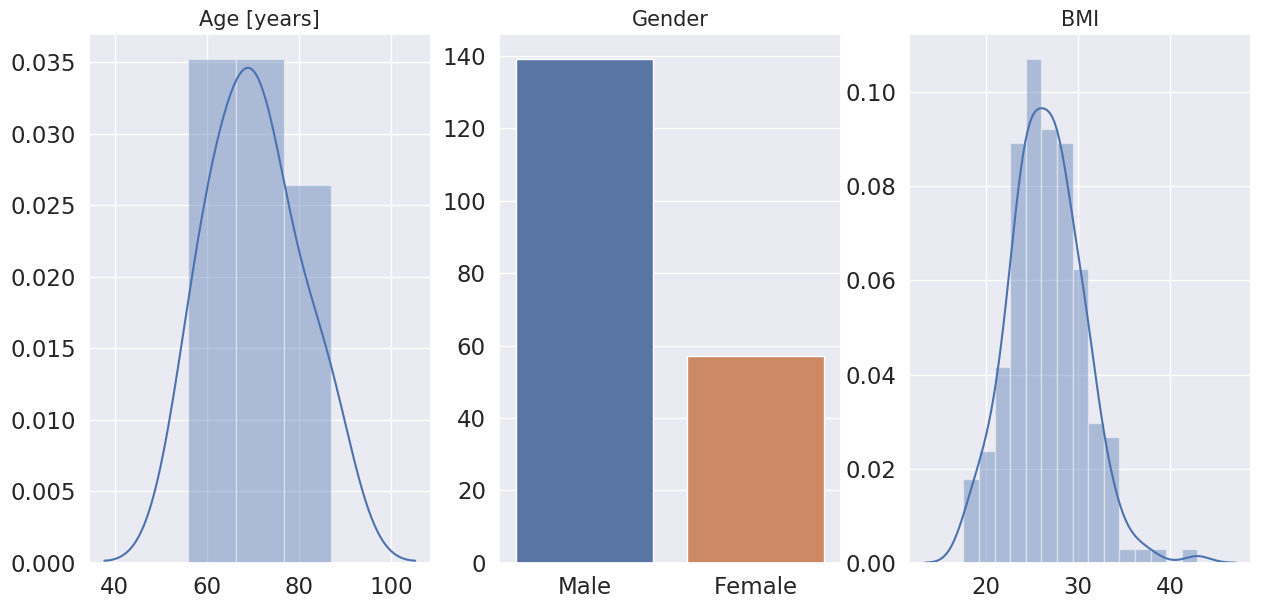
\includegraphics[width=\textwidth]{data-exp/metadataDist4.png}
    \end{center}
    \caption{Distribution of age, gender and BMI.}
    \label{fig:meta-dist4}
\end{figure}

\begin{figure}
    \begin{center}
    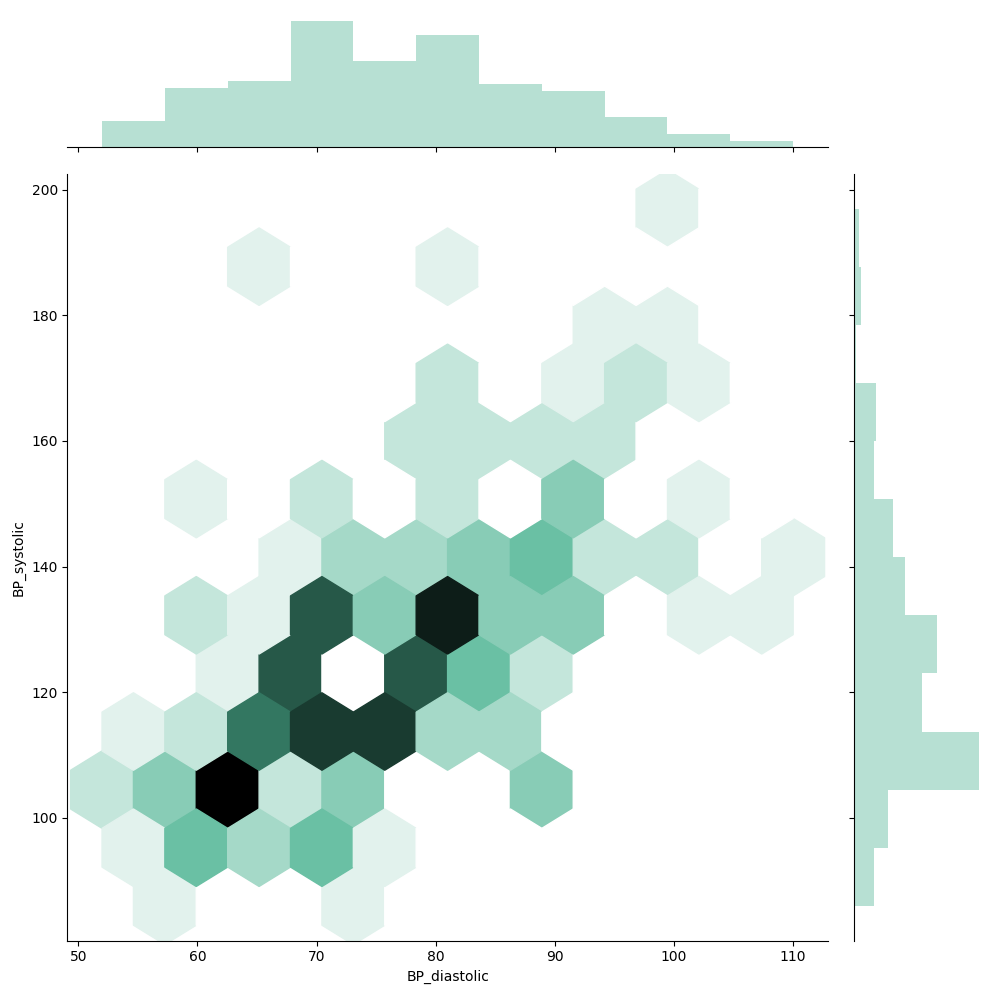
\includegraphics[width=0.4\textwidth]{data-exp/bp.png}
    \end{center}
    \caption{A joint distribtion plot of systolic and diastolic blood pressure of the patients.}
    \label{fig:bp-dist}
\end{figure}

Figure \ref{fig:meta-dist4} shows the patient distributions with regard to age, gender and BMI. As evident from the figure the patients that make up the dataset is made up of 138 males and 57 females. The majority of the patients are in the age group 60-80 years with a number of patients in the range 80-90 years (AGE SECTION SUBJECT TO CHANGE). The BMI distribution of patients is centered around 26 $kg/m^2$.Figure \ref{fig:bp-dist} shows the joint distribution of systolic and diastolic blood pressure among the patients.

\section{Input variables} \label{sec:covariates}
As mentioned earlier in section REF the different machine learning models that will be applied will apply two types of input data, time-series data in the form of longitudinal strain curves, and point-values in the form of peak systolic global longitudinal strain and patient EF.

\subsection{Peak-values}

\begin{figure}
    \begin{center}
    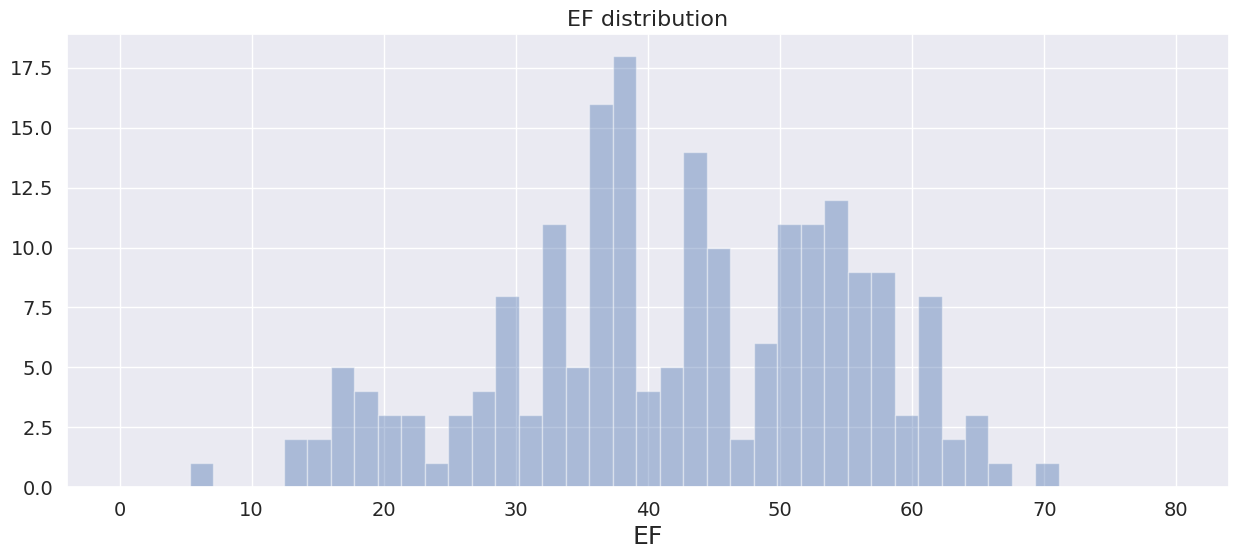
\includegraphics[width=0.4\textwidth]{data-exp/EF_dist.png}
    \end{center}
    \caption{Distribution of patient EF values.}
    \label{fig:}
\end{figure}

\begin{figure}
    \begin{center}
    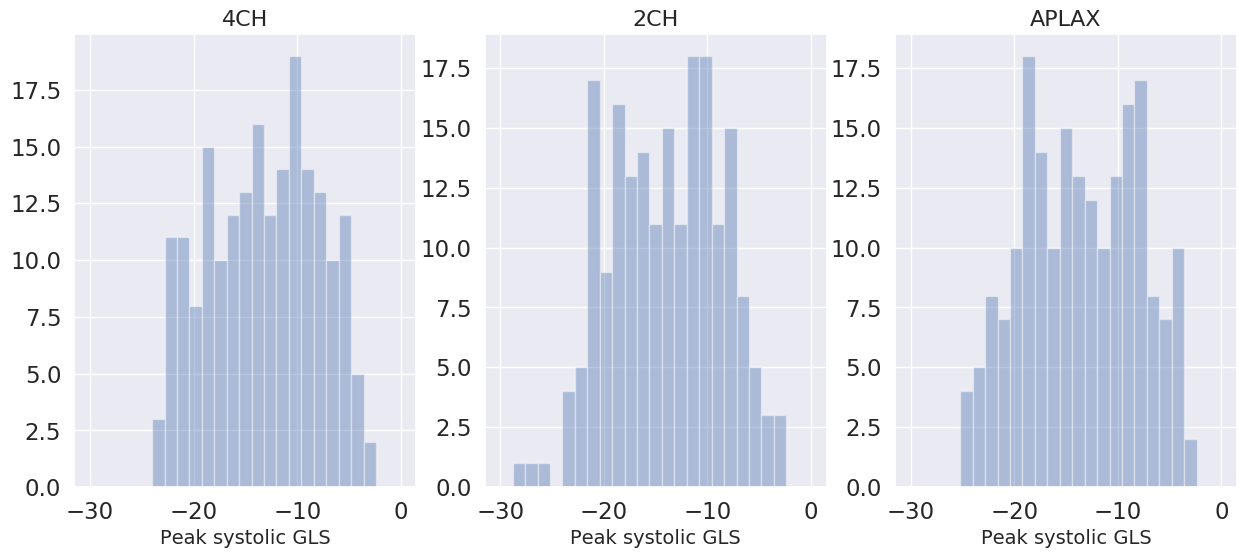
\includegraphics[width=0.4\textwidth]{data-exp/peak_sys_gls_dist.png}
    \end{center}
    \caption{Distribution of peak systolic global longitudinal strain.}
    \label{fig:}
\end{figure}

\subsection{Strain curves}

\begin{figure}
    \begin{center}
    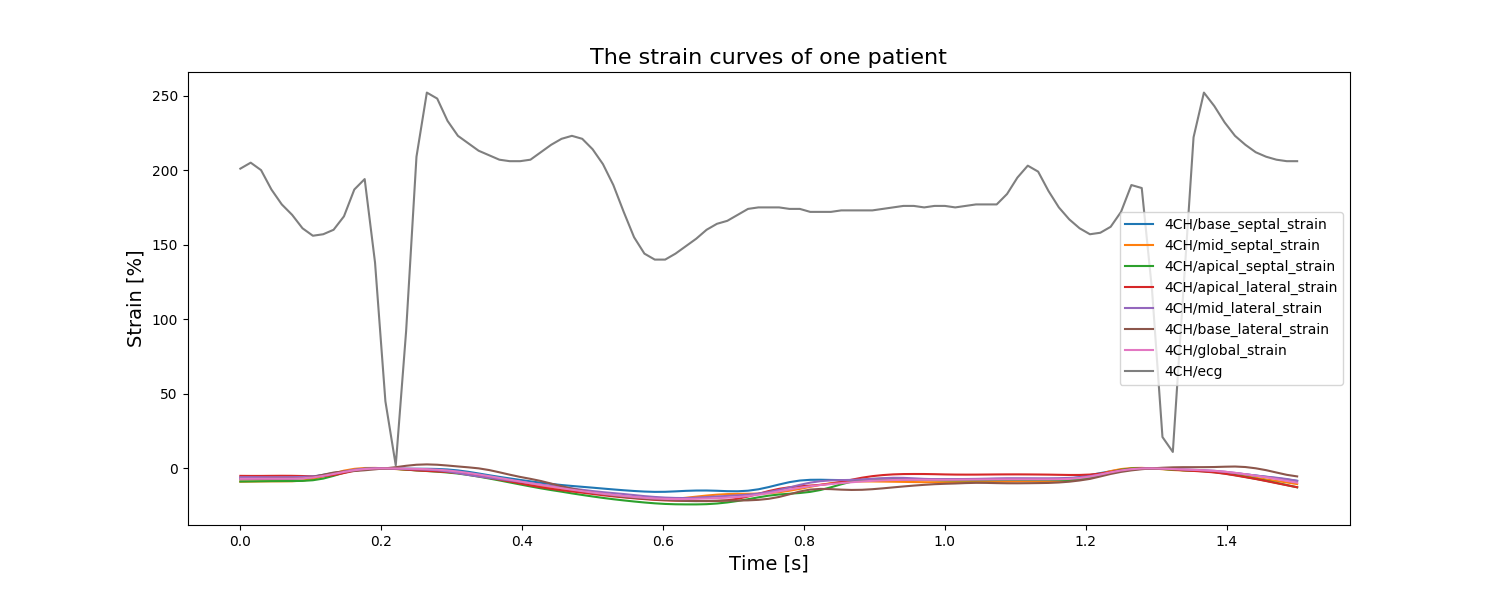
\includegraphics[width=0.4\textwidth]{data-exp/patient_strain_curves.png}
    \end{center}
    \caption{Plot of the global and regional longitudinal strain curves of one patient in the 4CH view.}
    \label{fig:}
\end{figure}

\section{Target variables} \label{sec:target}

\begin{figure}
    \begin{center}
    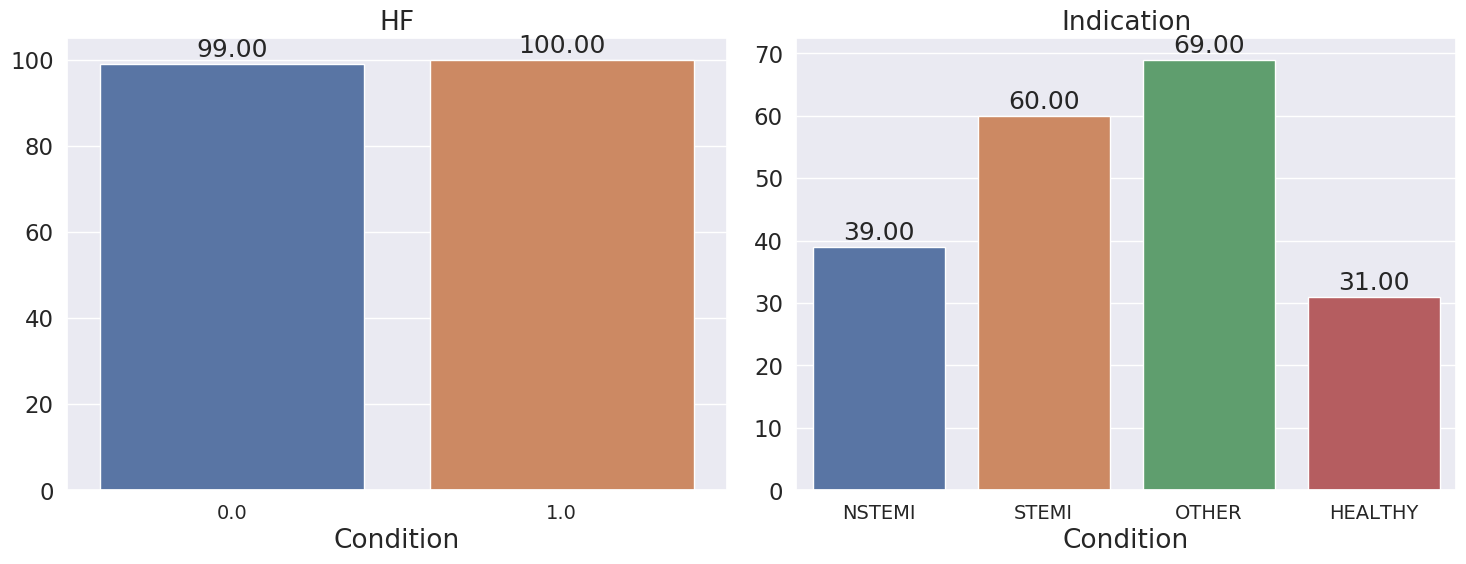
\includegraphics[width=0.4\textwidth]{data-exp/hf_indication_dist.png}
    \end{center}
    \caption{Distribution of heart failure within patients.}
    \label{fig:}
\end{figure}

\begin{figure}
    \begin{center}
    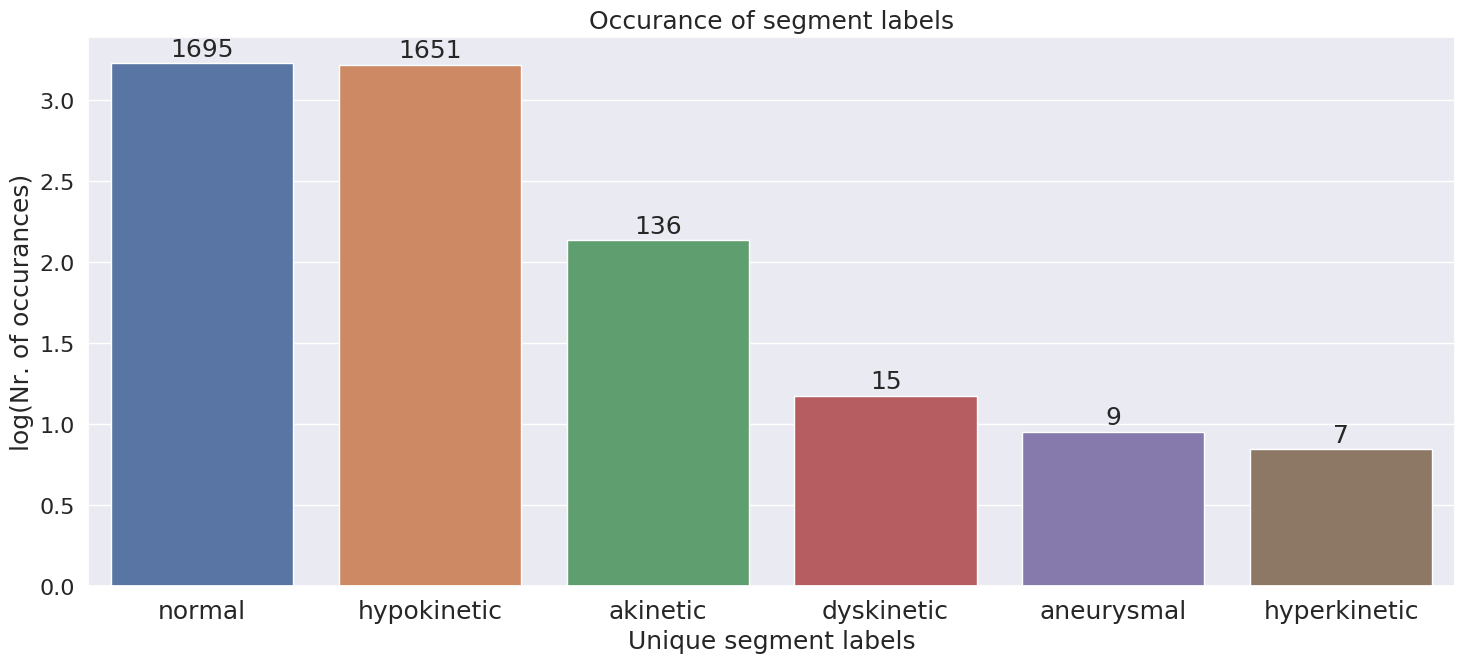
\includegraphics[width=0.4\textwidth]{data-exp/segment_label_distribution.png}
    \end{center}
    \caption{Distribution segment indication labels.}
    \label{fig:}
\end{figure}
